%%
%%
%% The first command in your LaTeX source must be the \documentclass
%% command.
%%
%% For submission and review of your manuscript please change the
%% command to \documentclass[manuscript, screen, review]{acmart}.
%%
%% When submitting camera ready or to TAPS, please change the command
%% to \documentclass[sigconf]{acmart} or whichever template is required
%% for your publication.
%%
%%
\documentclass[sigconf,screen,review,anonymous]{acmart}

\usepackage{multirow}
\usepackage{svg}
\usepackage{xcolor}
\usepackage{hyperref}
\usepackage{bbding}
\usepackage{courier}


\newcommand{\todo}[1]{\textcolor{red}{\textbf{[TODO:#1]}}}

%%
%% \BibTeX command to typeset BibTeX logo in the docs
\AtBeginDocument{%
  \providecommand\BibTeX{{%
    Bib\TeX}}}

%% Rights management information.  This information is sent to you
%% when you complete the rights form.  These commands have SAMPLE
%% values in them; it is your responsibility as an author to replace
%% the commands and values with those provided to you when you
%% complete the rights form.
\setcopyright{acmcopyright}
\copyrightyear{2024}
\acmYear{2024}
\acmDOI{XXXXXXX.XXXXXXX}

%% These commands are for a PROCEEDINGS abstract or paper.
\acmConference[FSE '24]{The 32nd ACM Symposium on the Foundations of Software Engineering}{November 15--19, 2024}{Porto de Galinhas, Brazil}
%%
%%  Uncomment \acmBooktitle if the title of the proceedings is different
%%  from ``Proceedings of ...''!
%%
\acmBooktitle{Proceedings of the 32nd ACM Symposium on the Foundations of Software Engineering (FSE '24), November 15--19, 2024, Porto de Galinhas, Brazil}
\acmPrice{15.00}
\acmISBN{978-1-4503-XXXX-X/18/06}


\settopmatter{printacmref=false}
\renewcommand\footnotetextcopyrightpermission[1]{}

%%
%% Submission ID.
%% Use this when submitting an article to a sponsored event. You'll
%% receive a unique submission ID from the organizers
%% of the event, and this ID should be used as the parameter to this command.
%%\acmSubmissionID{123-A56-BU3}

%%
%% For managing citations, it is recommended to use bibliography
%% files in BibTeX format.
%%
%% You can then either use BibTeX with the ACM-Reference-Format style,
%% or BibLaTeX with the acmnumeric or acmauthoryear sytles, that include
%% support for advanced citation of software artefact from the
%% biblatex-software package, also separately available on CTAN.
%%
%% Look at the sample-*-biblatex.tex files for templates showcasing
%% the biblatex styles.
%%

%%
%% The majority of ACM publications use numbered citations and
%% references.  The command \citestyle{authoryear} switches to the
%% "author year" style.
%%
%% If you are preparing content for an event
%% sponsored by ACM SIGGRAPH, you must use the "author year" style of
%% citations and references.
%% Uncommenting
%% the next command will enable that style.
%%\citestyle{acmauthoryear}


%%
%% end of the preamble, start of the body of the document source.
\begin{document}

%%
%% The "title" command has an optional parameter,
%% allowing the author to define a "short title" to be used in page headers.
\title{RAX:Efficiently Evaluating the Complexity of Porting for RISC-V}

%%
%% The "author" command and its associated commands are used to define
%% the authors and their affiliations.
%% Of note is the shared affiliation of the first two authors, and the
%% "authornote" and "authornotemark" commands
%% used to denote shared contribution to the research.
\author{Yuxuan Wang}
\email{wangyuxuan22@otcaix.iscas.ac.cn}
\affiliation{%
  \institution{Institute of Software, Chinese Academy of Sciences}
  \city{Haidian}
  \state{Beijing}
  \country{China}
}

%%
%% By default, the full list of authors will be used in the page
%% headers. Often, this list is too long, and will overlap
%% other information printed in the page headers. This command allows
%% the author to define a more concise list
%% of authors' names for this purpose.
\renewcommand{\shortauthors}{Yuxuan et al.}

%%
%% The abstract is a short summary of the work to be presented in the
%% article.
\begin{abstract}
  In recent years, the open-source and the advantages of reduced ISA of the RISC-V architecture are attracting active promotion of porting within the industry.Due to the lack of public available standards for assessing software portability, the software porting process for the RISC-V architecture has been predominantly reliant on expert experience, which is inefficient and time consuming. RAX is a automated tool which aids the C/C++ programmer in evaluating  complexity of software during porting for RISC-V.RAX provides precise evaluation solutions and builds a high-quality dataset for porting complexity,enabling recommendations of suitable software with difficulty levels for developers of varying skill levels.We evaluate RAX on 72 popular and typical real-scenario C/C++ projects. The experimental result shows that 51 of them have been confirmed by developers within community.Interested users can explore the open-source implementation of RAX at \href{https://github.com/wangyuliu/RAX-2024}{https://github.com/wangyuliu/RAX-2024}, or watch the RAX video demo at \href{https://www.youtube.com/watch?v=SLphW3Ra4WM}{https://www.youtube.com/watch?v\\=SLphW3Ra4WM}.
\end{abstract}

%%
%% The code below is generated by the tool at http://dl.acm.org/ccs.cfm.
%% Please copy and paste the code instead of the example below.
%%
\begin{CCSXML}
<ccs2012>
    <concept>
        <concept_id>10011007.10011006.10011072</concept_id>
        <concept_desc>Software and its engineering~Software libraries and repositories</concept_desc>
        <concept_significance>500</concept_significance>
        </concept>
    <concept>
        <concept_id>10011007.10011074.10011111</concept_id>
        <concept_desc>Software and its engineering~Software post-development issues</concept_desc>
        <concept_significance>300</concept_significance>
    </concept>
</ccs2012>
\end{CCSXML}
  
\ccsdesc[500]{Software and its engineering~Software libraries and repositories}
\ccsdesc[300]{Software and its engineering~Software post-development issues}


%%
%% Keywords. The author(s) should pick words that accurately describe
%% the work being presented. Separate the keywords with commas.
\keywords{ISA(Instruction set architecture), RISC-V, Porting Complexity Evaluation}

%% A "teaser" image appears between the author and affiliation
%% information and the body of the document, and typically spans the
%% page.
%% \begin{teaserfigure}
%%  \includegraphics[width=\textwidth]{sampleteaser}
%%  \caption{Seattle Mariners at Spring Training, 2010.}
%%  \Description{Enjoying the baseball game from the third-base
%%  seats. Ichiro Suzuki preparing to bat.}
%%  \label{fig:teaser}
%% \end{teaserfigure}

%% \received{20 February 2007}
%% \received[revised]{12 March 2009}
%% \received[accepted]{5 June 2009}

%%
%% This command processes the author and affiliation and title
%% information and builds the first part of the formatted document.
\maketitle

\section{Introduction}
RISC-V Instruction Set Architecture (ISA) has garnered significant attention from academia, and particularly the industry recently, due to its open-source and reduced design\citep{2014The}.Many distribution manufacturers are actively promoting the porting of the RISC-V, for example,OpenEuler has joined RISC-V International organization, and RISC-V has officially become openEuler's official support architecture.The main repository of openEuler 23.03 has successfully ported 4,244 software packages to the RISCV64,while the openEuler 23.09 main repository has currently completed the porting work of 5,694 software packages\citep{osti_1560132}.OpenCloudOS Kernel Stream 2207.2 kernel version adds support for the RISC-V 64 architecture\citep{osti_1560133}.  

Despite the rapid development of the RISC-V ISA, which foundational software such as operating systems and compilers are relatively mature, there is still a significant demand for porting a large number of application software\citep{2019Notary}.To adapt to the RISC-V,efficiently porting is greatly depending on prior knowledge of experts, and the lack of standardized evaluation criteria for software portability can lead to unreasonable development planning.Therefore, it is desirable to propose a method that automates the evaluation of porting complexity.This will enable different development teams to access software packages that are tailored to their abilities, thus assisting distribution vendors in the porting of RISC-V architecture.  

Many related works focus on the code complexity and portability evaluation,but studies for CPU architectures are currently lacking in these areas\cite{2016helei},\cite{TAHIR2016101},\cite{Sholiq_2021}.Du et al. have developed a basic statistical evaluation plan for CPU architecture code\citep{2023du}.However,their work lacks a thorough validity analysis of factors,and may not consider the complexity factors associated with the software operation and maintenance process.
To overcome these challenges, we propose RAX, an effective porting
complexity evaluation tool which accurately locates the CPU architecture code and calculates the code complexity of the software.The contributions of this paper are as follows:
\begin{itemize}
  \item We analysis the actual porting modifications and figure out one of the most important factors,Cyclomatic Complexity(CC), exploring its significant value in porting scenarios.
  % \item We explore building high-quality datasets that can cover various porting scenarios to solve the problem of imbalanced datasets of existing tools.Tuning machine learning models to address ambiguous identification of samples of medium and hard complexity compared to other studies.
  \item Based on architecture-related factors, we propose RAX, to efficiently assess the complexity of software during porting to the RISC-V.
  % \item We nearly doubled the dataset compared to other tool,and verified the effectiveness of the evaluation of 51 extension projects in real porting scenarios through their respective communities or forums.Our findings indicate that RAX outperforms other tool, delivering substantial improvements in terms of accuracy.
  \item We build a dataset of real-world C/C++ projects and use it to evaluate the effectiveness of RAX.Our findings indicate that RAX outperforms other tool, delivering substantial improvements in terms of accuracy.
\end{itemize}
The remainder of this paper is organized as follows.In Section 2,we briefly analyze architecture-related factors. Section 3 presents the implementation and evaluation of RAX. Section 4 and 5 presents related work and conclusions.

% \section{RAX}
% The following is an introduction to the process of RAX construction, as shown in Figure \ref{fig:figure1}.
% During the analysis phase,architecture-related factors are obtained through the Commit tool for selection while investigating the impact of code complexity metrics on porting.
% A scanning tool is built to get potential modification workload.
% Finally,an appropriate machine learning model is selected as a classification.
% \begin{figure}
%   \centering
%   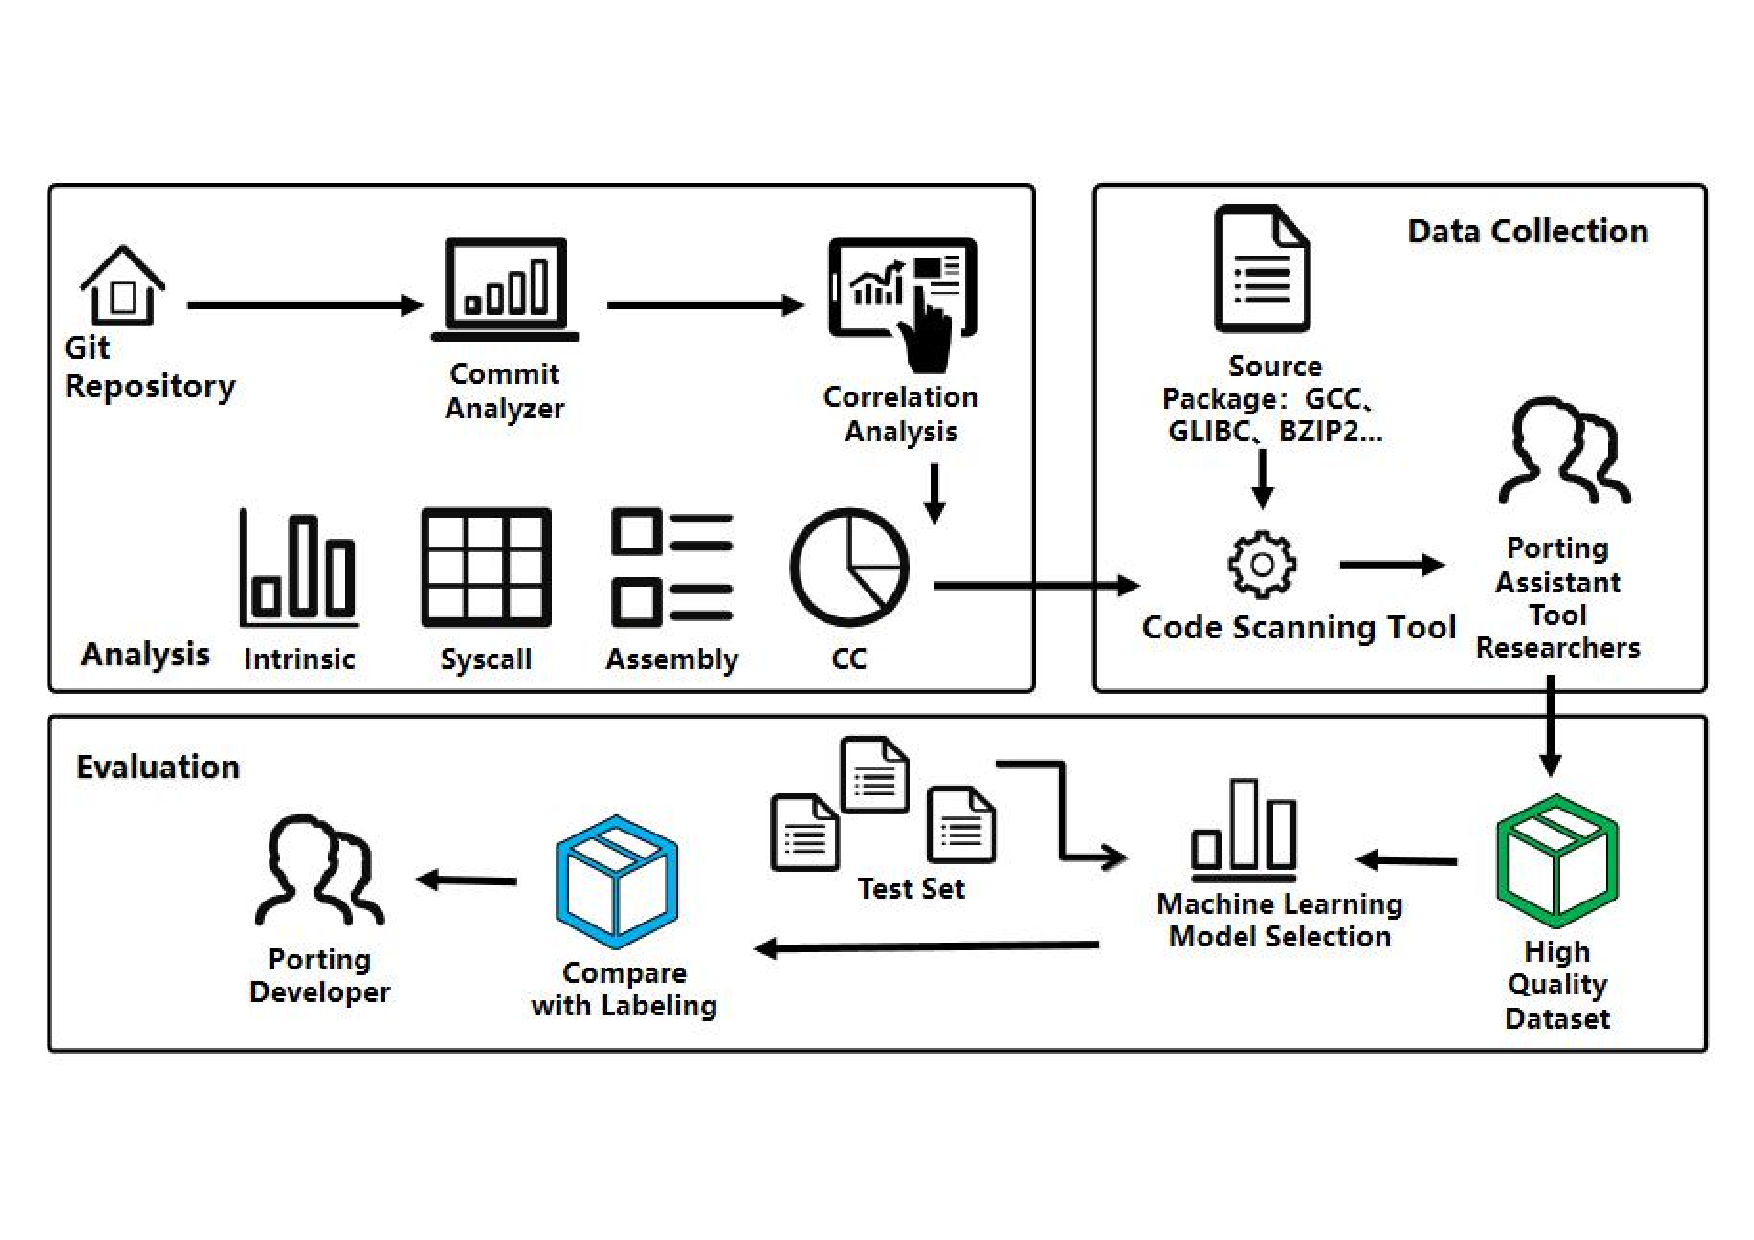
\includegraphics[width=\linewidth]{figure1.pdf}
%   \caption{Flow chart for method to build RAX}
%   \label{fig:figure1}
%   \Description{Flow chart for method to build RAX}
% \end{figure}
\section{Motivation}
\label{sec:factor}
To help developers more accurately assess the porting complexity of C/C++ projects, we aim to answer the following research questions:

\textbf{RQ 1:} How can we select architecture-relevant factors that is fine-grained to design an automated evaluation tool of porting complexity?

\textbf{RQ 2:} How to implement fine-grained and automated tools to help developers accurately assess the complexity of their projects in real world?\\
As we all known, the metrics of projects porting complexity is influenced by many factors, such as the scale of projects,the logical structure of the architectural code. To answer RQ 1, we introduce the code Cyclomatic Complexity(CC) and Arch\_code.
% \begin{figure}
%   \centering
%   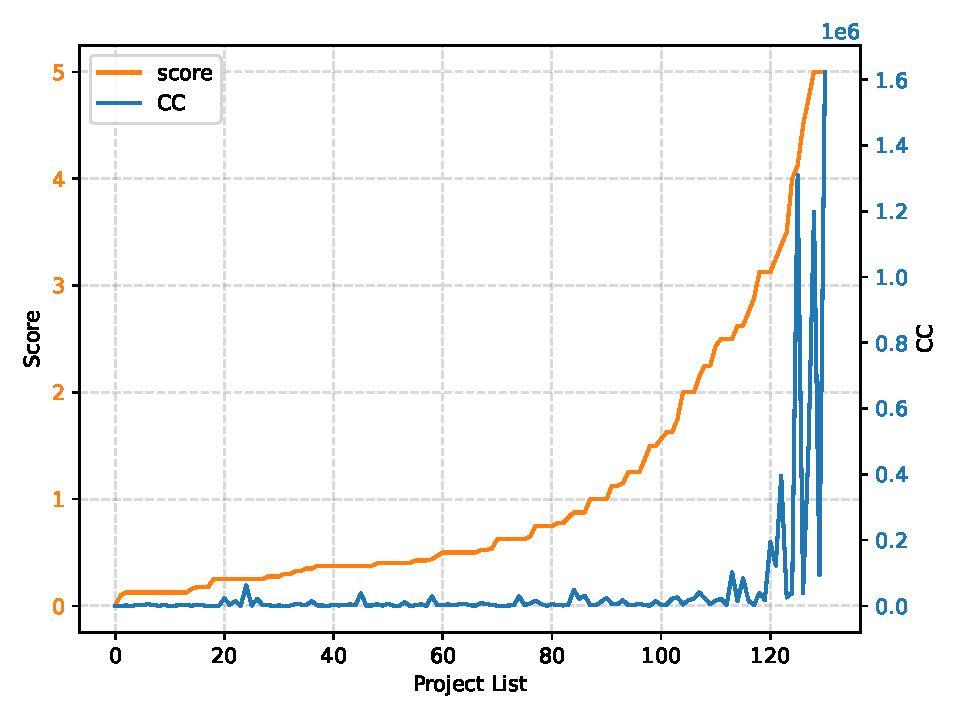
\includegraphics[width=\linewidth]{figure2.pdf}
%   \caption{The relationship between score and CC}
%   \label{fig:figure2}
%   \Description{The relationship between score and CC}
% \end{figure}
 
% To answer RQ 1,this section provides a validity analysis of porting-related factors on RAX.
% First,we try to use code complexity metrics to evaluate porting work.
% The software metrics of code Cyclomatic Complexity(CC) can help developers make macro judgments on software complexity and maintenance difficulty. By evaluating potential and hidden porting difficulties,code complexity helps the tool improve accuracy \cite{2005Exploring}.
% At present, CC indicators are mostly used in evaluating code quality, inspecting defect, reconstructing code, etc \cite{1991Cyclomatic}.
% During the porting process, developers will target a large number of project source codes,build scripts,assembly codes,and a macro understanding of the project is required in the early stage of porting.
% This part of the work has a lot of overlap with the scope of code complexity.Through our survey of community, we discovered that even though architectural code can be separated quite clearly from common code, when faced with large-scale projects, we still require numerous iterative tests to uncover unknown architectural code. Building upon this, we study the quantification of the significance of cyclomatic complexity in porting work.
\begin{figure}
  \centering
  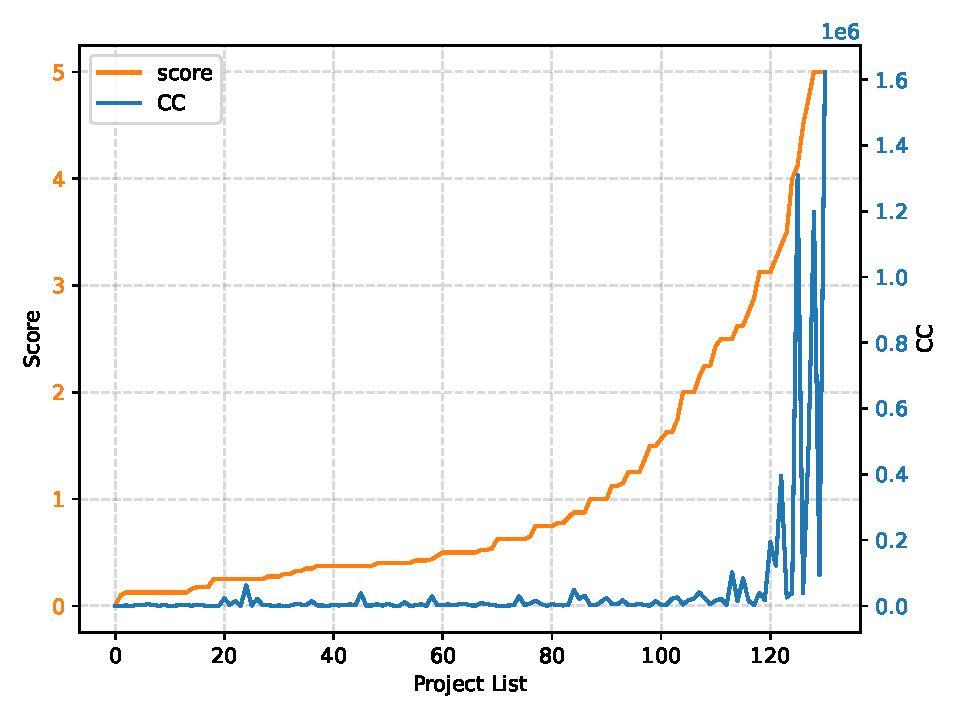
\includegraphics[width=\linewidth]{figure2.pdf}
  \caption{The Relationship between Score and CC}
  \label{fig:figure2}
  \Description{The Relationship between Score and CC}
\end{figure}
\subsection{Factor 1: Cyclomatic Complex(CC)}
\label{sec:factor-1}
First,we try to use code complexity metrics to evaluate porting work.
CC can help developers make macro judgments on software complexity and maintenance difficulty,and helps the tool improve accuracy \cite{2005Exploring}.
% At present, CC indicators are mostly used in evaluating code quality, inspecting defect, reconstructing code, etc \cite{1991Cyclomatic}.
During the porting process, developers will target a large number of project source codes,and a macro understanding of the project is required in the early stage of porting.This part of the work has a lot of overlap with the scope of code complexity.Through our survey of community, we discovered that even though architectural code can be separated quite clearly from common code, when faced with large-scale projects, we still require numerous iterative tests to uncover unknown architectural code.
Based on the above, we use the lizard CC detection tool and optimize its functions.This paper proposes a new CC method:
 First, we calculate the function-level CC for all files in the project using McCabe's method. Following Liu's mention of System Cyclomatic Complexity (SCC) in software evolution assessment techniques based on code change detection \cite{liuhuihui00}, we define SCC as the total sum of function-level values in the system.
  Our CC calculation approach is expressed by equation (1) to (3),where lowercase cc represents the cyclomatic complexity at the function or file level.The uppercase CC represents the overall cyclomatic complexity of the software package,serving as a crucial factor in our tool.Here, |E| denotes the number of edges in the function control flow graph,and |N| represents the number of nodes.The function control flow graph is constructed based on branching structures such as if, while, and switch statements. 
  
  \begin{equation}
    {cc}({function}) = \lvert E \rvert - \lvert N \rvert + 2
    % \sum_{i=1}^{n} x_i
    \end{equation}
    \begin{equation}
      {cc}({file}) =  \sum_{i=1}^{n} 
      {cc}({function})
      \end{equation}
      \begin{equation}
        {CC} =  \sum_{i=1}^{k} {cc}({file})
        \end{equation}
this section calculate the correlation coefficient using the Spearman Rank.
We invited five Master's students who are engaged in research on porting auxiliary tools to score the porting complexity(score) of 131 projects adapted for RISC-V,collected from the OpenEuler list\citep{stage2023} and GitHub.
According to the collection of Internet events, log analysis, source code dismantling, and similar project analogy \cite{liangguanyu2020}, we form a scoring interval in the range of $[0,5]$.
The Spearman coefficient of CC and score is 0.608, with a P-value of 1.39e-14, which is less than 0.01.
The results suggest that CC has a moderate positive correlation with porting difficulty.
This is because developers need a holistic understanding of the project during the porting process, and CC can represent the overall complexity of the project, potentially reflecting porting barriers, the relationship of factors shown in Figure \ref{fig:figure2}.




Second, we consider the effectiveness of the architecture-related code structure proposed by other tool and conduct comparative experiments using more potential factors.
\begin{figure}
  \centering
  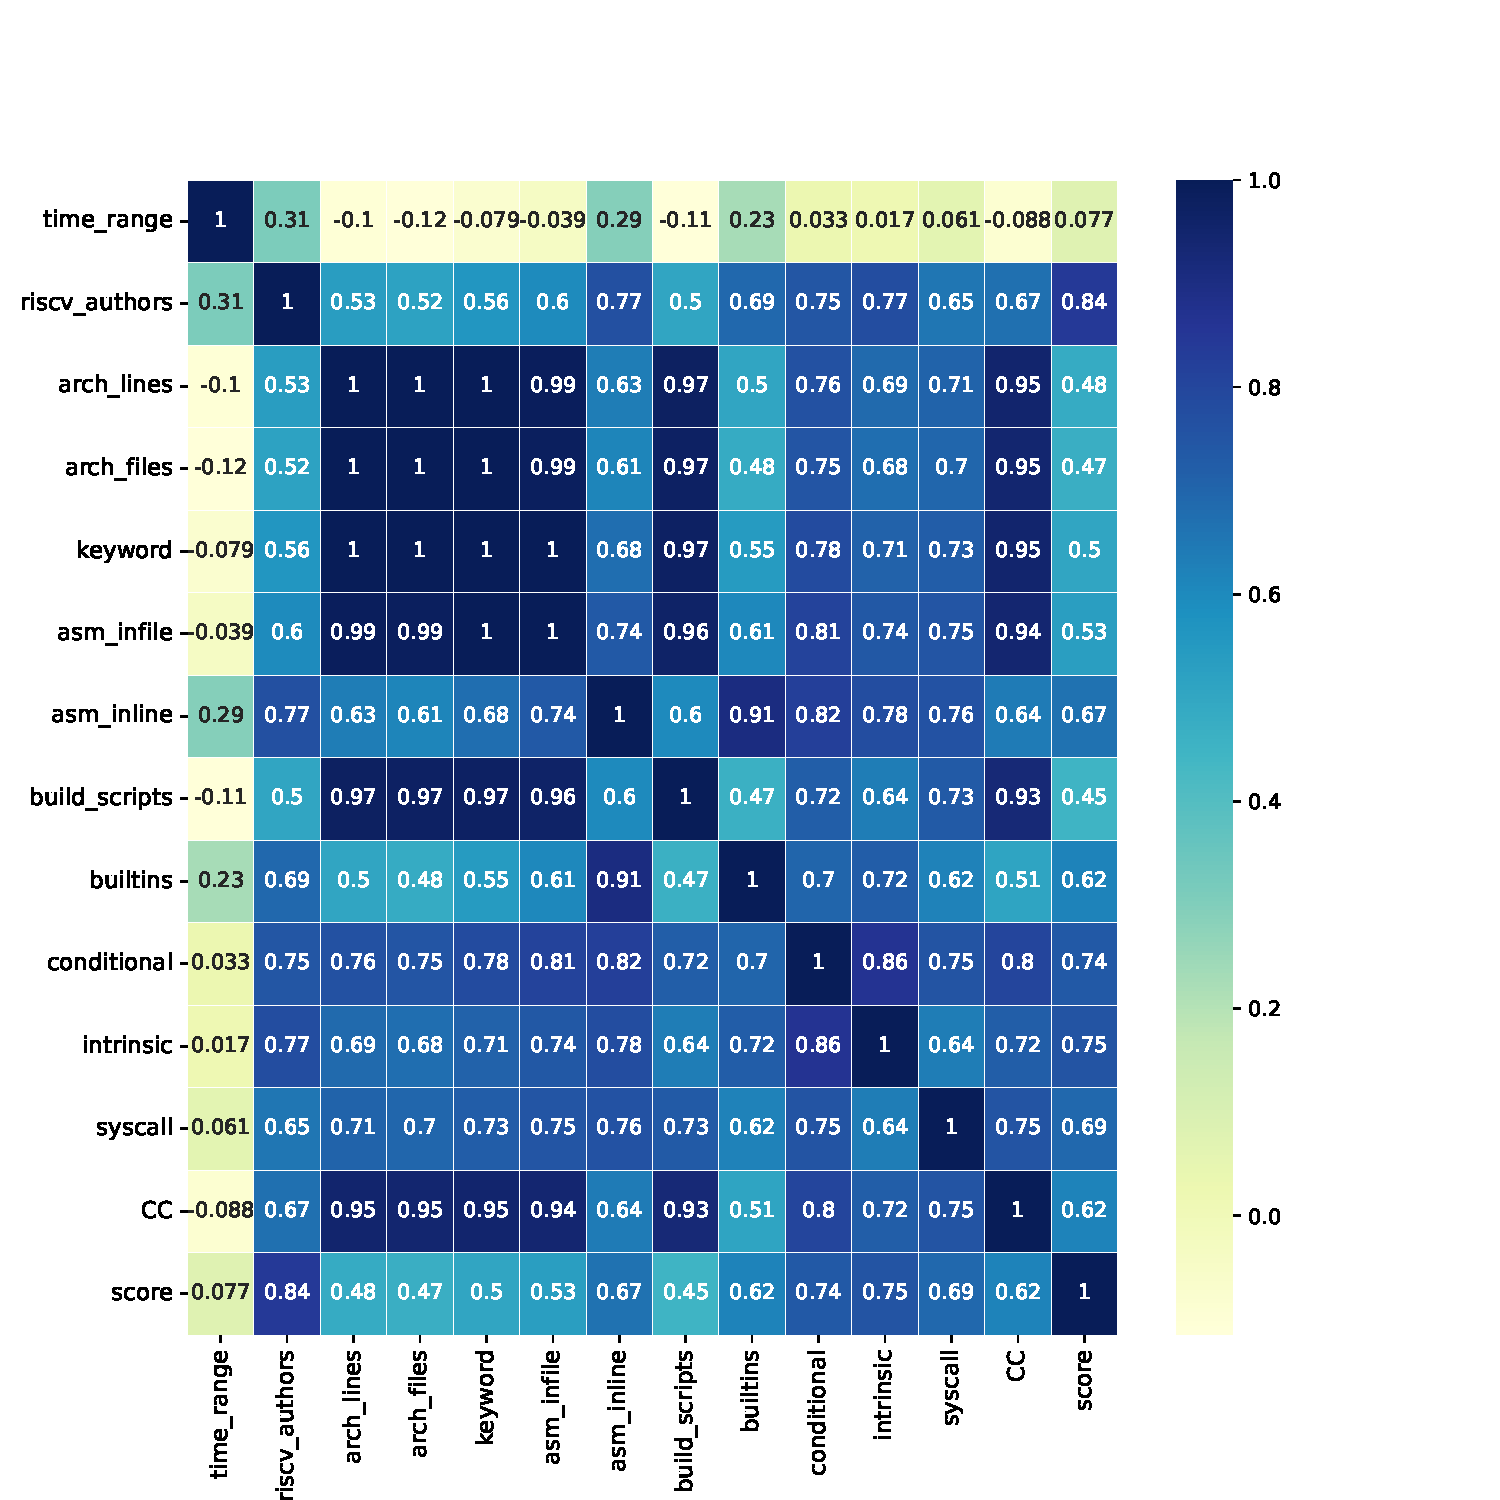
\includegraphics[width=\linewidth]{figure3.pdf}
  \caption{The Heat Map of Pearson Correlation}
  \label{fig:figure3}
  \Description{The Correlation}
\end{figure}
\subsection{Factor2:Arch\_code}

We select factors with the greatest potential from existing tool and define Arch\_code.
Arch\_code includes assembly code, conditional compilation and macro structure(CCM), Intrinsic functions, Builtin functions, architecture-related build scripts, and system calls.
We use an automated tool to obtain statistics of lines and frequencies of Arch\_code.
We form the Arch\_code dictionary:
(1)\textit{Conditional compilation and architecture macros} Use conditional compilation statements, such as ``\texttt{if defined}'', ``\texttt{ifdef}'', in conjunction with all possible architecture macros,
  ``\texttt{\_\_x86\_64\_\_}''.
  We use an algorithm similar to bracket matching to cover all the code within macros, avoiding the impact of nested layers.
  (2)\textit{Assembly} We use matching forms such as ``\texttt{\_\_asm\_\_}'' and ``\texttt{\_\_volatile\_\_}''.
  In future work,we will consider striving to achieve the currently unachievable architecture identification function of assembly code;
  (3)\textit{Intrinsic and Builtin} 
  We compile dictionaries of Intrinsic and Builtin functions based on official documentation from x86\cite{x86intrin}.In the future,we may assign difficulty weights to them.
  (4)\textit{System calls} The system calls that do not support RISC-V have been filtered and collected currently.
  (5)\textit{Buildscripts} We locate architecture keywords in the build scripts.


We further collect other factors that may reflect the porting complexity,and select the following parameters through the Commit analyzer:architecture-related code lines, architecture-related files, and architecture keywords.architecture-related code lines and files is located using the keywords of the RISC-V architecture, such as riscv, rv32, rv64, RISC-V, RISCV and so on.
%Correlation comparison between Arch\_code and other factors acquired by Commit analyzer,as shown in Table \ref{tab:Tool}:

%\begin{table}
 % \caption{The Spearman correlation coefficient of score and architecture-related factors}
  %\label{tab:score}
  %\begin{tabular}{cc}
   % \toprule
    %Type & Score \\
    %\midrule
    %conditional compilation & 0.73 \\
    %Builtin & 0.61 \\
    %Intrinstic & 0.74 \\
    %syscall & 0.69 \\
    %asm & 0.66 \\
    %build\_scripts & 0.43 \\
    %time & -0.16 \\
    %authors & 0.43 \\
    %lines of arch & 0.16-0.40 \\
    %files of arch & 0.34-0.41 \\
    %keyword count & 0.17-0.43 \\
   % \bottomrule
  %\end{tabular}
%\end{table}


\begin{table*}
  \centering
  \caption{Factors Among Different Tools}
 %% \resizebox{0.48\textwidth}{!}{
  \label{tab:Tool}
  \begin{tabular}{ccccccccc}
    \toprule
    & Full Assembly & Inline Assembly & Intrinsic & Builtin & System Call & CCM & Buildscripts & CC \\
    \midrule
   Tool\citep{2023du} & \CheckmarkBold & \CheckmarkBold & \CheckmarkBold & \CheckmarkBold & \CheckmarkBold & \CheckmarkBold & \CheckmarkBold & \XSolidBrush \\
    RAX & \CheckmarkBold & \CheckmarkBold & \CheckmarkBold & \CheckmarkBold & \CheckmarkBold & \CheckmarkBold & \CheckmarkBold & \CheckmarkBold \\
  \bottomrule
\end{tabular}
 %% }
\end{table*}


Figure \ref{fig:figure3} shows the correlation comparison between Arch\_code,CC and other factors acquired by Commit analyzer:The results indicate that Arch\_code and CC has a higher correlation with score compared to other factors, and we use Peason correlation method to build the heat map.
The use of only architecture keywords for statistics yields moderate effectiveness because keywords can only be detected from comments and macro sections of Git commits, while critical porting code may lack these keywords,but the number of keywords can reflect the amount of porting modification from the side.
Arch\_code show a correlation of 0.45 to 0.75 with score, indicating a strong relationship.
However, using a single factor alone does not result in a significantly strong correlation, as the combined modifications of these factors make up the porting workload.

In the end,our tool selection was CC and the Arch\_code build scanning tool,as shown in Table \ref{tab:Tool}.

% To design RAX that assists developers with porting work,the following research questions are proposed:

% \textbf{RQ 1:} How can we select architecture-relevant actors that is fine-grained to design an automated tool that assesses the porting difficulty?

% \textbf{RQ 2:} How to select a classifier to obtain effective classification results for the tool?


% \begin{table}
%   \caption{Tool factors comparison table}
%   \label{tab:comparisons}
%   \begin{tabular}{ccccc}
%     \toprule
%     Porting Complexity & \multicolumn{2}{c}{Du's Tool} & \multicolumn{2}{c}{RAX} \\
%      & TP & FN & TP & FN \\
%     \midrule
%     Low &32/37 & 5/37 & 35/37 & 2/37 \\
%     Medium & 5/8 & 3/8 & 6/8 & 2/8 \\
%     High & 2/6 & 4/6 & 6/6 & 0/6 \\
%     \midrule
%     Total & \textcolor{red}{39/51} & 12/51& \textcolor{red}{47/51} & 4/51 \\
%       \bottomrule
% \end{tabular}
% \end{table}
% \documentclass{article}
% \usepackage{pifont} % 加载pifont宏包

% \begin{table*}
%   \caption{Tool factors comparison}
%   \label{tab:Tool}
%   \begin{tabular}{ccccccccc}
%     \toprule
%     & Full Assembly & Inline Assembly & Intrinsic & Builtin & System Call & Conditional compilation and macro & Buildscripts & CC \\
%     \midrule
%     Toolone & \checkmark & \checkmark & \checkmark & \checkmark & \checkmark & \checkmark & \checkmark & \\
%     RAX & \checkmark & \checkmark & \checkmark & \checkmark & \checkmark & \checkmark & \checkmark & \checkmark \\
%   \bottomrule
% \end{tabular}
% \end{table*}


% \begin{table*}
%   \caption{The Spearman correlation coefficient of score and architecture-related factors}
%   \label{tab:score}
%   \begin{tabular}{cccccc}
%     \toprule
%     conditional compilation & Builtin & Intrinstic & syscall & asm & build\_scripts \\
%     \midrule
%     0.73 & 0.61 & 0.74 & 0.69 & 0.66 & 0.43 \\
%   \bottomrule
% \end{tabular}
% \begin{tabular}{ccccc}
%   \toprule
%   time & authors & lines of arch & files of arch & keyword count \\
%   \midrule
%   -0.16 & 0.43 & 0.16-0.40 & 0.34-0.41 & 0.17-0.43 \\
% \bottomrule
% \end{tabular}
% \end{table*}


% \begin{table}
%   \caption{Tool factors comparison}
%   \label{tab:comparisont}
%   \begin{tabular}{ccccc}
%     \toprule
%      & Accuracy & Pmacro & Rmacro & F1macro \\
%     \midrule
%     Adaboost & 0.786 & 0.594 & 0.775 & 0.650 \\
%     Random Forest & \textcolor{red}{0.857} & 0.817 & 0.873 & 0.836 \\
%   \bottomrule
% \end{tabular}
% \end{table}

\section{RAX}
Since we identify architecture-relevant important factors affecting porting efficiency, we implement a fine-grained and automated tool to evaluate complexity. Figure \ref{fig:figure1} shows the entire technology roadmap in three parts such as Analysis, Data Collection and {Evaluation. RAX can be deployed easily by installing dependencies, highlighting its convenience and user-friendliness.

% \textcolor{blue}{The following is an introduction to the process of RAX construction, as shown in Figure \ref{fig:figure1}.
% During the analysis phase,architecture\-related factors are obtained through the Commit tool for selection while investigating the impact of code complexity metrics on porting.
% A scanning tool is built to get potential modification workload. Finally,an appropriate machine learning model is selected as a classification.}

\begin{figure}
  \centering
  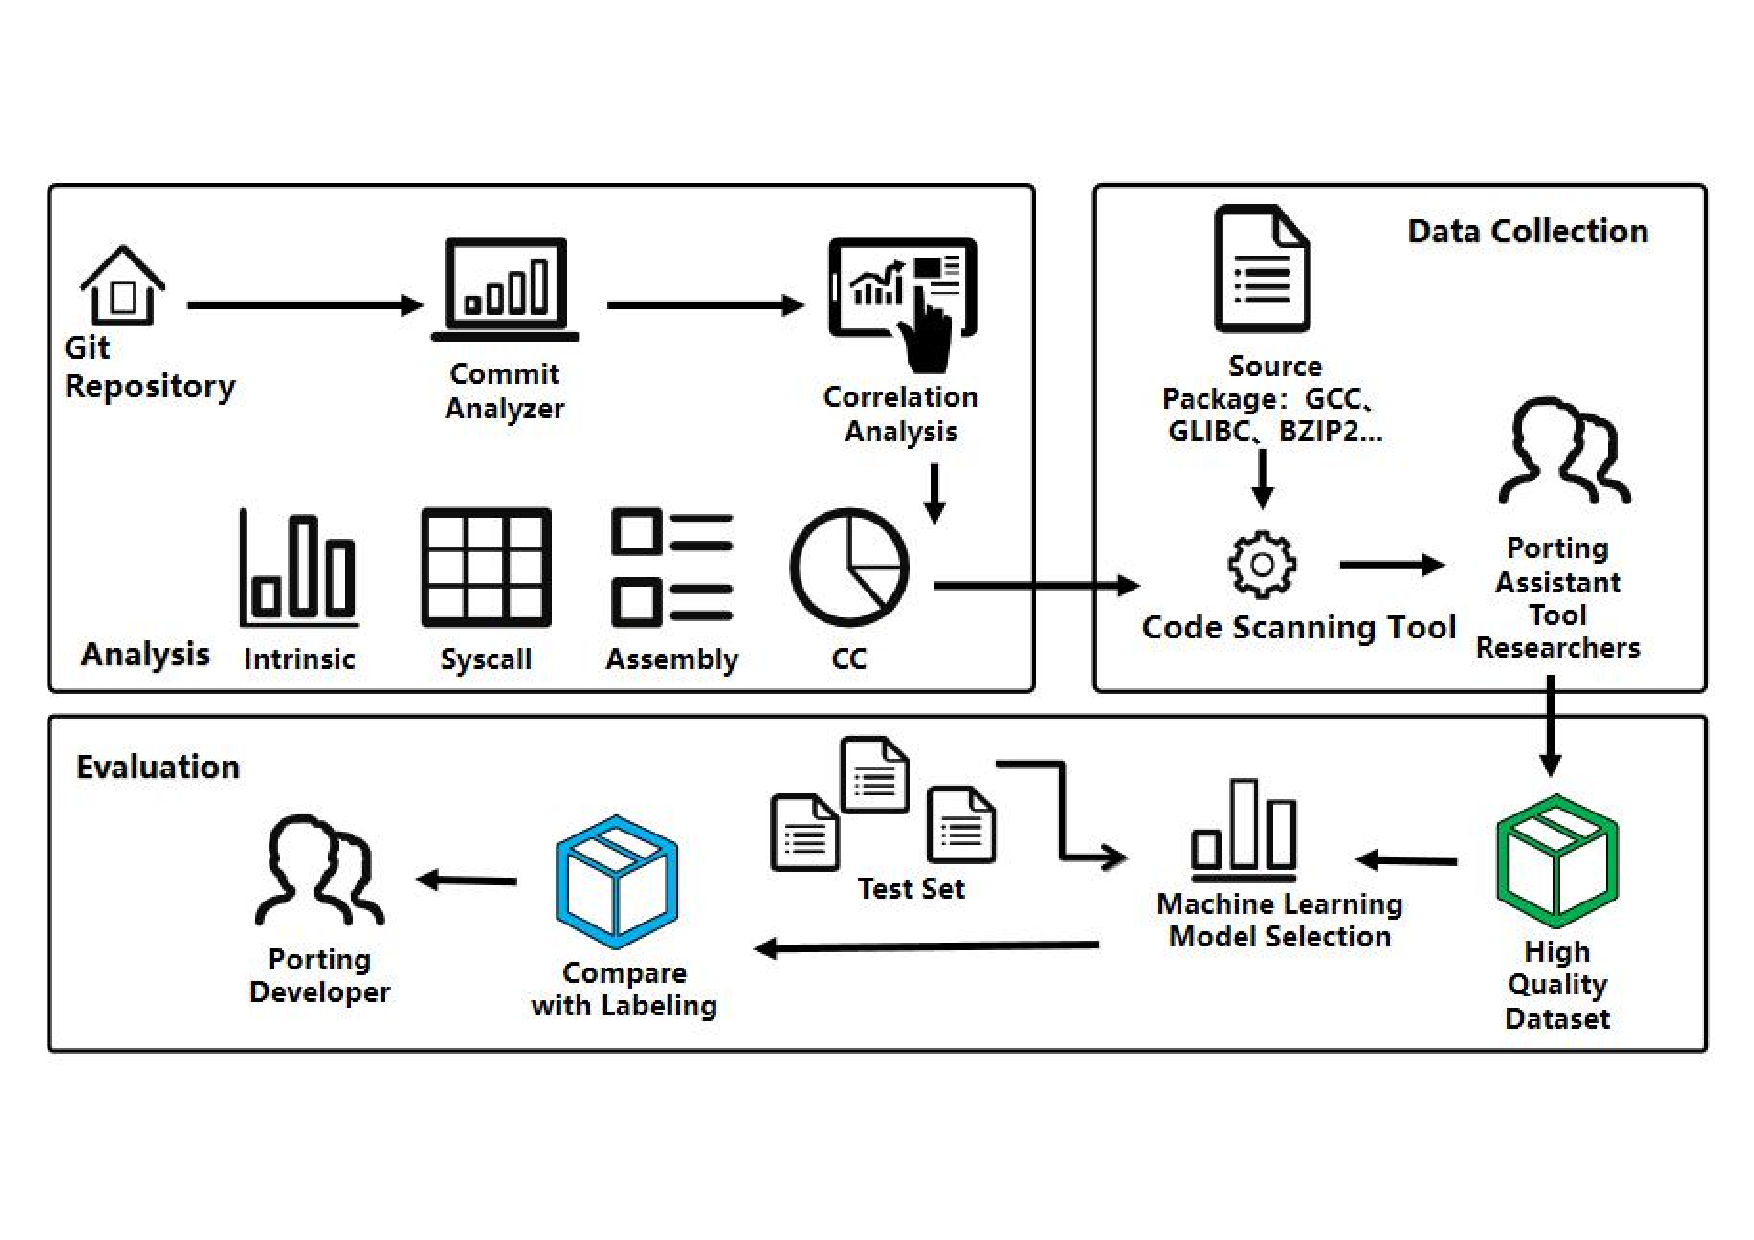
\includegraphics[width=\linewidth]{figure1.pdf}
  \caption{Flow Chart of RAX}
  \label{fig:figure1}
  \Description{Flow Chart for Method to Build RAX}
\end{figure}

% \subsection{Dataset}
% We used the project upstream warehouse to build the data set,that projects mainly targeting C and C++ are from the OpenEuler list and GitHub,and invited 5 postgraduate students who are engaged in the research of RISC-V porting auxiliary tools to participate in the experimental evaluation.Specific evaluation methods can be found in \ref{sec:factor-1}. The evaluation scores are divided into three categories: low, medium, and high\citep{githuburl}.This includes 139 projects as training, testing, and validation datasets, while more than 80 additional projects were used as a tool effectiveness evaluation dataset. To gather insights from developers, the community, forums, and emails were utilized, resulting in over 51 meaningful feedback responses. In order to address the issue of data imbalance caused by collecting datasets solely from the openEuler mailing list, where more than 80\% of the projects were initially evaluated as having low porting complexity, a greater emphasis was placed on projects that had higher numbers of likes on GitHub and were deemed more important and active. Additionally, efforts were made to collect projects from the system bottom such as operating systems, kernel-level projects,mathematical computation libraries,and machine learning libraries to address RQ 2.

\subsection{Implementation}
\label{sec:Implementation}
% RAX obtains porting complexity vector through the CC calculation method and Arch\_code statistical value.
\subsubsection{Analysis}
We intend to use the Lizard tool, which employs a methodology consistent with the McCabe's method\cite{1702388}, to obtain CC metrics.
However, Lizard tool only defects at the function level and uses the average function CC for file-level statistics, which is not suitable for current porting complexity detection requirements \cite{9402593}.We need to redefine the CC method to avoid the use of complex methods, which will cause deviations to affect the classification results.Additionally, we must address the potential performance overhead problem caused by converting the entire project into abstract syntax tree.\\
Other tools only consider x86 architecture to locate architecture-related code for statistical analysis. We propose a new idea that explore whether multiple architectures can be selected or if other architectures can be individually targeted. Based on this, we conducted comparative experiments using various architectures, including X86, ARM, MIPS, RISCV, SPARC, and PowerPC. We performed scanning and counting based on the keyword and function dictionaries specific to each architecture, which were derived from common patterns summarized by official websites.
By analyzing the correlation coefficient (Pearson's) between the keyword coverage line statistics of the six architectures and the score representing the porting complexity, we found that the correlation ranged from 0.44 to 0.58, indicating all correlation results are not significant. Additionally, the correlation between the total values for all architectures and score was only 0.49.
Based on these results, analyze that our tool try to effectively assess the porting difficulty between two architectures. It is not as simple as adding up the modification amounts for different architectures, as it may only reflect an increase in code volume. Moreover, due to the large differences in row-based statistical results caused by the differences in code structure reflected by each architecture, this approach that easily considers all architectures simultaneously without considering the code structure and architectural weight lead to ambiguous outcomes.Therefore, based on these experiments, we still select x86 to build Arch\_code scan function, given its mainstream position.
\subsubsection{Dataset Collection}
% We used the project upstream warehouse to build the data set,which mainly targeting C and C++ are from the OpenEu-ler list and GitHub,and invited 5 postgraduate students who are engaged in the research of RISC-V porting auxiliary tools to participate in the experimental evaluation.Specific evaluation methods can be found in \ref{sec:factor-1}. The evaluation scores are divided into three categories: low, medium, and high\citep{githuburl}.This includes 139 projects as training, testing, and validation datasets, while 72 additional projects were used as a tool effectiveness evaluation dataset. To gather insights from developers, the community, forums, and emails were utilized, resulting in over 51 meaningful feedback responses. 

We used the project upstream warehouse to build the data set,which mainly targeting C and C++ are from the OpenEuler list and GitHub\citep{stage2023}.In order to address the issue of data imbalance caused by collecting datasets solely from the openEuler mailing list, where more than 80\% of the projects were initially evaluated as having low porting complexity, a greater emphasis was placed on projects that had higher numbers of likes on GitHub and were deemed more important and active. Additionally, efforts were made to collect projects from the system bottom such as operating systems, kernel-level projects,mathematical computation libraries,and machine learning libraries. It is worth emphasizing that, all these projects' complexity evaluated by RAX hoped to be verified  by the own developer of projects.

\subsubsection{Evaluation}
% RAX obtains porting complexity vector through the CC calculation method and Arch\_code statistical value.\\
% This paper proposes a new CC method:
%  First, we calculate the function-level CC for all files in the project using McCabe's method. Following Liu's mention of System Cyclomatic Complexity (SCC) in software evolution assessment techniques based on code change detection \cite{liuhuihui00}, we define SCC as the total sum of function-level values in the system.
%   Our CC calculation approach is expressed by equation (1) to (3),where lowercase cc represents the cyclomatic complexity at the function or file level.The uppercase CC represents the overall cyclomatic complexity of the software package,serving as a crucial factor in our tool.Here, |E| denotes the number of edges in the function control flow graph,and |N| represents the number of nodes.The function control flow graph is constructed based on branching structures such as if, while, and switch statements. 
  
%   \begin{equation}
%     {cc}({function}) = \lvert E \rvert - \lvert N \rvert + 2
%     % \sum_{i=1}^{n} x_i
%     \end{equation}
%     \begin{equation}
%       {cc}({file}) =  \sum_{i=1}^{n} 
%       {cc}({function})
%       \end{equation}
%       \begin{equation}
%         {CC} =  \sum_{i=1}^{k} {cc}({file})
%         \end{equation}
% We form the Arch\_code dictionary:
% (1)\textit{Conditional compilation and architecture macros} Use conditional compilation statements, such as ``\texttt{if defined}'', ``\texttt{ifdef}'', in conjunction with all possible architecture macros,
%   ``\texttt{\_\_x86\_64\_\_}''.
%   We use an algorithm similar to bracket matching to cover all the code within macros, avoiding the impact of nested layers.
%   (2)\textit{Assembly} We use matching forms such as ``\texttt{\_\_asm\_\_}'' and ``\texttt{\_\_volatile\_\_}''.
%   In future work,we will consider striving to achieve the currently unachievable architecture identification function of assembly code and identify assembly code in the form of instructions;
%   (3)\textit{Intrinsic and Builtin} 
%   We compile dictionaries of Intrinsic and Builtin functions based on official documentation from x86\cite{x86intrin}.In the future,we may assign difficulty weights to them.
%   (4)\textit{System calls} Considering glibc's support for system call encapsulation, reorganize the sys-call dictionary.
%   The system calls that do not support RISC-V have been filtered and collected currently.
%   (5)\textit{Buildscripts} We locate architecture keywords in the build scripts.
In our study, we opted to utilize Random Forest machine learning model for conducting training and testing to obtain the final classifier model. The extended dataset was used as an additional input for the classifier to acquire evaluation results. We subsequently performed evaluations on 72 projects and sought community feedback during the tool's effectiveness evaluation phase.


% \subsubsection{Arch\_code scan function}
% Other tools only consider x86 architecture to locate architecture-related code for statistical analysis. We propose a new idea that explore whether multiple architectures can be selected or if other architectures can be individually targeted. Based on this, we conducted comparative experiments using various architectures, including X86, ARM, MIPS, RISCV, SPARC, and PowerPC. We performed scanning and counting based on the keyword and function dictionaries specific to each architecture, which were derived from common patterns summarized by official websites.
% By analyzing the correlation coefficient (Pearson's) between the keyword coverage line statistics of the six architectures and the score representing the porting complexity, we found that the correlation ranged from 0.44 to 0.58, indicating all correlation results are not significant. Additionally, the correlation between the total values for all architectures and score was only 0.49.
% Based on these results, analyze that our tool try to effectively assess the porting difficulty between two architectures. It is not as simple as adding up the modification amounts for different architectures, as it may only reflect an increase in code volume. Moreover, due to the large differences in row-based statistical results caused by the differences in code structure reflected by each architecture, this approach that easily considers all architectures simultaneously without considering the code structure and architectural weight lead to ambiguous outcomes.Therefore, based on these experiments, we still select x86 to build Arch\_code scan function, given its mainstream position.

% We form the Arch\_code dictionary:
% (1)\textit{Conditional compilation and architecture macros} Use conditional compilation statements, such as ``\texttt{if defined}'', ``\texttt{ifdef}'', in conjunction with all possible architecture macros,
%   ``\texttt{\_\_x86\_64\_\_}''.
%   We use an algorithm similar to bracket matching to cover all the code within macros, avoiding the impact of nested layers.
%   (2)\textit{Assembly} We use matching forms such as ``\texttt{\_\_asm\_\_}'' and ``\texttt{\_\_volatile\_\_}''.
%   In future work,we will consider striving to achieve the currently unachievable architecture identification function of assembly code and identify assembly code in the form of instructions;
%   (3)\textit{Intrinsic and Builtin} 
%   We compile dictionaries of Intrinsic and Builtin functions based on official documentation from x86\cite{x86intrin}.In the future,we may assign difficulty weights to them.
%   (4)\textit{System calls} Considering glibc's support for system call encapsulation, reorganize the sys-call dictionary.
%   The system calls that do not support RISC-V have been filtered and collected currently.
%   (5)\textit{Buildscripts} We locate architecture keywords in the build scripts.
 
\subsection{Evaluation}
\subsubsection{Dataset}
 To evaluate RAX, We chose typical and popular C and C++ projects from upstream warehouse of the OpenEuler and GitHub\citep{stage2023}. First, we searched keywords "rv" or "riscv" and collected 139 projects as our training and testing dataset. Then, five postgraduate students are invited to tag the porting auxiliary for these projects. The evaluation scores are divided into three categories:low, medium, and high\citep{githubss}. Second, models are trained and tested based on the 139 projects. Third, to evaluate the RAX, additional 72 projects are collected and evaluated from GitHub. To gather response from developers, the community, forums, and emails were utilized. 
\subsubsection{Result and Analysis}
To solve the problem of unbalanced datasets and small sample datasets, we used ensemble learning methods \cite{6509481}, SMOTE \cite{4271036}, and random oversampling methods for data preprocessing\cite{5128907} addressing.By comparing multiple indicators, we select the Random Forest, which had the highest accuracy of 0.857 as the classifier, as shown in Table \ref{tab:evaluation}.

\begin{table}
  \caption{Experimental Results of Models}
  \label{tab:evaluation}
  \begin{tabular}{ccccc}
    \toprule
     & Accuracy & Pmacro & Rmacro & F1macro \\
    \midrule
    Adaboost & 0.786 & 0.594 & 0.775 & 0.650 \\
    Random Forest & \textcolor{red}{0.857} & 0.817 & 0.873 & 0.836 \\
  \bottomrule
\end{tabular}
\end{table}

We provide a comprehensive compilation of the community's valuable feedback comments, accompanied by the relevant web links for further reference and validation shown in \cite{githubss} and Table \ref{tab:effectiveness}. Our experiments shows that, compared with other tool, RAX is more accurately to evaluate projects' complexity. In detail, the true positive (TP) of other tool is 39/51, while the RAX is 47/51.  At the same time, the RAX has a lower rate of false positive (FN) than other tools. The values are 4/51 and 12/51, respectively. Through real-world evaluations within the developer community, our tool has exhibited a significant improvement in accuracy, surpassing other comparable tools by a margin of 15.6\%. 

\begin{table}
  \caption{Tool Effectiveness Comparison from Community Feedback}
  \label{tab:effectiveness}
  \begin{tabular}{ccccc}
    \toprule
    Porting Complexity & \multicolumn{2}{c}{Du's Tool} & \multicolumn{2}{c}{RAX} \\
     & TP & FN & TP & FN \\
    \midrule
    Low &32/37 & 5/37 & 35/37 & 2/37 \\
    Medium & 5/8 & 3/8 & 6/8 & 2/8 \\
    High & 2/6 & 4/6 & 6/6 & 0/6 \\
    \midrule
    Total & \textcolor{red}{39/51} & 12/51& \textcolor{red}{47/51} & 4/51 \\
      \bottomrule
\end{tabular}
\end{table}

After adding the code complexity factor and modifying the original model, RAX's result prediction accuracy is improved.
This is because code complexity can clearly distinguish three types of porting difficulty.
Motivation Chapters present the cause analysis.
Adding factors also makes RAX more robust and more friendly to projects with unbalanced complexity vectors.
For example, kernel-level projects, boot layers, hardware drivers and other projects may involve a large amount of assembly code,corresponding to larger porting complexity,but other factors of the original tool design are at low values,which is not conducive to distinguishing complexity.
Chibios,u-boot are facing such a situation. Another reason is that we have added more medium or difficult complex samples to the data set to increase robustness and improve the innovativeness of the tool. Within evaluation, there are instances of inaccurate predictions. Analysis of some variations reveals that certain projects exhibit inherent complexity, entailing a substantial presence of architecture-specific code defined by Arch\_code.
Nevertheless, the practical porting process benefits from an array of auxiliary tools designed to support developers. In response to valuable suggestions from developers within the OpenEuler community, we conducted an evaluation of the porting complexity for various versions of the Chromium.Initially, we were able to accurately assess the porting complexity, yielding promising results. However, when it came to evaluating the work involved in iterative updates between versions, existing tools proved insufficient for precise estimation.Sometimes CPU architecture parts in projects are well separated from the common code,that just need only to adjust the moderate amount of code to recognize RISC-V,like nuttx.
\section{Related Work}
With the development of the RISC-V ecosystem,  projects of porting for RISC-V has attracted much attention in both academia and industry. For example,Tine Blaise et al.\cite{osti_1830102} accomplished the porting of the OpenCL framework to commodity RISC-V, thereby expanding RISC-V's accessibility to a wider range of scientific computing applications.
Cao Hao et al.\cite{2017Slow}designed an automated porting framework to solve the problem of efficient porting of basic mathematics libraries.
However,there is still a lack of fine-grained assistance tools for architecture portability evaluation.
% Our work consider code complexity from the perspective of its evaluation role in software evolution and maintenance,mapping its influence on porting complexity evaluation\cite{1993Software}.
Alvares et al. \cite{7844689} proposed using the development team's ``tolerance'' for code complexity to infer team development capabilities and performance indicators for projects.
Vard et al. \cite{2017Evaluating} emphasized that the internal quality of software impacts developers' capabilities and maintenance duration.
They conducted a comprehensive study on various existing code complexity metrics' validity and suggested incorporating empirically observed code features as complexity triggers.We have pioneered the application of code complexity metrics in the domain of porting assessment, while existing research primarily focuses on code refactoring and defect detection\cite{1993Software},\cite{1991Cyclomatic}.
\section{Conclusion}
The software porting work for RISC-V is being actively promoted, but it still faces the challenge of over-reliance on expert knowledge.We propose RAX, with the aim of recommending projects of varying porting difficulties to developers. Our method incorporate the code complexity and architectural code to reflect developers' actual workload. We verified the effectiveness of the evaluation of 51 extension projects in real porting scenarios through their respective communities or forums. Observed significant performance improvements compared to existing tools.Moreover, RAX provides developers with the functionality to locate target code segments.Our next steps involve attempting text classification methods and designing more granular statistical methods for architecture-related factors.
%%
%% The acknowledgments section is defined using the "acks" environment
%% (and NOT an unnumbered section). This ensures the proper
%% identification of the section in the article metadata, and the
%% consistent spelling of the heading.
\begin{acks}
  This work was supported by the Strategic Priority Research Program of the Chinese Academy of Sciences (Grant No. XDA0320102) and Youth Innovation Promotion Association, Chinese Academy of Sciences (Grant No. 2023118).
\end{acks}

%%
%% The next two lines define the bibliography style to be used, and
%% the bibliography file.
\bibliographystyle{ACM-Reference-Format}
\bibliography{paper}



\end{document}